\documentclass[12pt,a4paper]{article}
\usepackage[latin1]{inputenc}
\usepackage{amsmath}
\usepackage{amsfonts}
\usepackage{amssymb}
\usepackage{makeidx}
\usepackage{graphicx}
\usepackage{mhchem}
\usepackage{textcomp}
\usepackage{booktabs}
\usepackage{mathrsfs,amsmath} 
\usepackage{steinmetz}
\usepackage{subcaption}
\usepackage{bm}
\usepackage{hhline}
\usepackage[left=2.00cm, right=2.00cm, top=2.00cm, bottom=2.00cm]{geometry}
\author{}
\title{\textbf{Preliminary}}	 
\date{}

\begin{document}
	\maketitle
	
	\section{Hardware}
	\subsection{Raspberry Pi 4 B}
	As a Microntroller, we'll be using a Raspberry Pi 4 model B of 2GB of ram memory, as illustrated in the Figure \ref{fig:RasPi}.
	
    \begin{figure}[h]
    	\centering
    	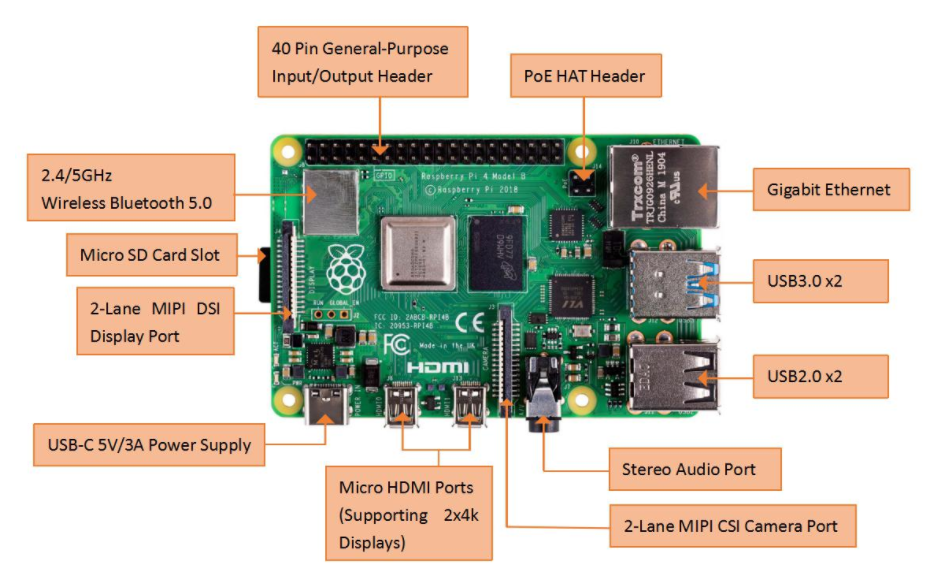
\includegraphics[width=0.7\linewidth]{Imm/RasPi-Definition}
    	\caption{\textit{Raspberry Pi 4 model B interfaces and GPIO.}}
    	\label{fig:RasPi}
    \end{figure}
    
    As we can see, we can interact with the raspi in different ways, in particular:
    \begin{itemize}
    	\item \textbf{USB-C Power Supply} of 5V/3A. For, we'll first use a AC Adapter as the one in Figure \ref{fig:Adapter} with an ON/OFF switch. 
    	
    	   \begin{figure}[h]
    	   	\centering
    	   	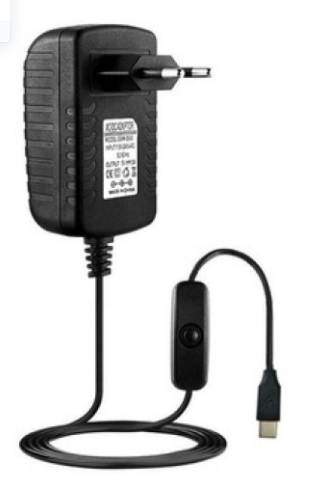
\includegraphics[width=0.2\linewidth]{Imm/Adapter}
    	   	\caption{\textit{AC Adapter for Power Supply of 5V/3A}}
    	   	\label{fig:Adapter}
    	   \end{figure}
    	   
    	Consequenly a stand alone battery will be used in order to make the car more autonomous.
    	\item \textbf{Micro HDMI Port} in order to connect the raspi to a screen thanks to a Micro HDMI-to-VGA adapter as in Figure \ref{fig: VGA-Adapter} (NOTE: this may change according to the screen, for instance mine has a VGA port) . Connecting the raspi on the screen will be usefull for the desktop configuration.
    	 \begin{figure}[h]
    	 	\centering
    	 	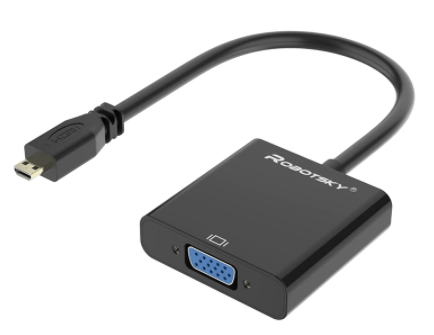
\includegraphics[width=0.2\linewidth]{Imm/VGA-Adapter}
    	 	\caption{\textit{Micro HDMI to VGA Adapter.}}
    	 	\label{fig: VGA-Adapter}
    	 \end{figure}
    	
    	\item \textbf{2-Lane MIPI CSI Camera Port} in order to connect the camera.
    	\item \textbf{Micro SD card slot} where we connect our 32 GB micro SD card flashed with the Operating System for the raspi (we'll see in Section 2 how to configure this).
    	\item \textbf{GPIO}, i.e. the General-Purpose Input/Outputs in order to interact with the different signals.
    \end{itemize}
    
    \subsection{4WD Smart Car Kit}
    The 4 Wheel-Drive Smart Car kit from Freenove includes the following components:
     \begin{figure}[h]
     	\centering
     	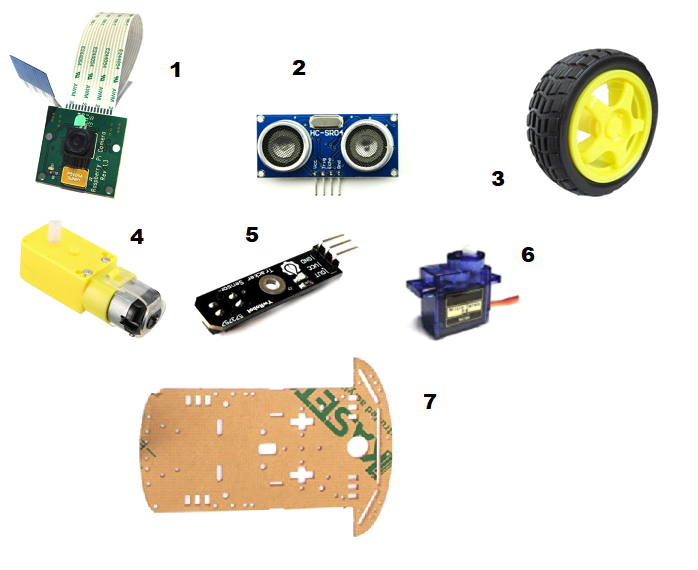
\includegraphics[width=0.6\linewidth]{Imm/Kit}
     	\caption{\textit{Smart car kit components.}}
     	\label{fig: Kit}
     \end{figure}
    \begin{enumerate}
    	\item \textbf{Car Chassis}
    	\item \textbf{4 Tire Wheels}
    	\item \textbf{4 DC Gear motors}
    	\item \textbf{2 Micro Servo motors 9g SG90}
    	\item \textbf{Raspberry Pi Camera Rev 1.3 module}
    	\item \textbf{Line Tracking Sensor}
    	\item \textbf{Ultrasonic Ranging module HC-SR04}
    \end{enumerate}
    	
    
	\section{Raspberry Pi Configuration}
	\section{Assembling}
	
\end{document}